\documentclass[main.tex]{subfiles}

\begin{document}

% \textcolor{red}{Вводная лекция}

\section{Лекция 02.03.2021 (Донцов Е.В.)}

\subsection{Из чего состоит любая модель ГРП? Продолжение}

Давайте вспомним предыдущую лекцию.

В модели ГРП \textbf{есть несколько основных концепций}, несколько основных физических процессов, которые необходимо описать и которые любой симулятор ГРП описывает (не важны тип геометрии, количество трещин, способ решения явный/неявный -- главное: учесть правильную физику/механику).

\textbf{Первое:} закон сохранения жидкости.
Предполагается, что она несжимаемая: закачиваем некий объём жидкости в скважину, часть этого объёма генерирует трещину и плюс часть жидкости утекает в виде утечек

\textbf{Второе:} градиент давления внутри трещины, который образуется из-за вязкого течения жидкости.

\textbf{Третье:} уравнение упругости.
Мы деформируем породу вокруг трещины; считаем породу линейно-упругим материалом; после деформаций должно выполняться условие равновесия.

\textbf{Четвёртое:} критерий распространения.
Аналогия с шариком: уравнение упругости показывает соотношение давления в шарике с его объёмом, а критерий распространения -- это условие при котором шарик лопнет.
То же самое с трещиной: упругость даёт нам соотношение между давлением жидкости внутри и открытием трещины, а критерий распространения позволяет найти условие, при котором трещина будет распространяться.

\textbf{Пятое:} транспорт проппанта.

В прошлый раз мы подробно остановились на модели утечек Картера и на уравнениях течения жидкости в трещине.
Сейчас продолжим говорить про упругость и критерии распространения.

\subsubsection{Равновесие (упругость) горной породы. Уравнение упругости}

\includegraphics[width=\textwidth, page=9]{HF_slides_2022.pdf}

Упругость: порода вокруг трещины должна быть в равновесии в зависимости от того, какое у трещины открытие или сдвиговое смещение в каждом элементе трещины.

В чём сложность расчёта теории упругости? В том, что этот процесс очень нелокальный.
Например, если у нас есть несколько трещин, несколько элементов (множество элементов в каждой трещине), то изменение открытия в каждом элементе влечёт за собой изменение поля напряжений во всём пространстве.
Т.е. если мы немного изменим степень открытости одного из элементов, то у нас будет влияние на все элементы.
С практической точки зрения коэффициент взаимодействия уменьшается довольно быстро с расстоянием ($\sim 1/r^3$ для трёхмерной геометрии).
Т.е. с точки зрения практики можем задать некий радиус, после которого будем обрезать взаимодействия.
Но тем не менее всё равно взаимодействие будет нелокальным.
В этом сложность упругости.


Для плоской трещины у нас есть довольно простое выражение.

Если рассматриваем плоскую трещину и двухмерную задачу, то давление в трещине равно сжимающему напряжению на бесконечности и плюс дополнительный интеграл от открытия трещины (как функции координаты) с сингулярным ядром.

Т.е. открытие в любой точке трещины влияет на давление по всей трещине.


Для планарной трещины есть более сложное выражение, которое выводится абсолютно аналогично выражению для плоской трещины.

Далее выведем выражение для плоской трещины; для планарной -- вывод такой же.


Я буду давать относительно простые примеры и относительно простые геометрии, но все рассматриваемые задачи решены и для сложных геометрий, и для полностью трёхмерных геометрий.

Вы можете найти все эти коэффициенты взаимодействия между элементами (интегральные ядра) для полностью трёхмерной задачи.

Всё, что я Вам покажу, верно для однородного по упругим свойствам материала.
Но в реальности могут быть геологические слои и модули упругости Юнга и коэффициенты Пуассона могут меняться от слоя к слою.

Если Вам не страшна жёсткая математика и Вы хотите посчитать коэффициенты взаимодействия между элементами в слоистой среде, то можете посмотреть статью Pierce и Siebrits.

Но нам в рамках курса важна общая концепция: откуда берутся выражения и что описывают с точки зрения физики/механики.

Давайте выведем уравнение упругости.
Что такое уравнение упругости?
Это условие того, что порода вблизи трещины находится в равновесии.
Мы рассматриваем плоскую трещину и вследствие симметрии рассматриваем половину задачи (только верхнюю часть трещины, например).

\includegraphics[width=\textwidth, page=10]{HF_slides_2022.pdf}

\subsubsection{Условие распространения трещины ГРП}

\includegraphics[width=\textwidth, page=11]{HF_slides_2022.pdf}

\includegraphics[width=\textwidth, page=12]{HF_slides_2022.pdf}

\includegraphics[width=\textwidth, page=13]{HF_slides_2022.pdf}

\subsection{Математическая модель планарной трещины ГРП (planar3D)}

\includegraphics[width=\textwidth, page=15]{HF_slides_2022.pdf}

Рассмотрим планарную трещину ГРП: трещина лежит в плоскости $Oxy$, раскрытие трещины по оси $Oz$.

Запишем закон сохранения объёма: новый объём есть старый объём плюс входящий поток по оси $Ox$ минус выходящий поток по оси $Ox$ плюс входящий поток по оси $Oy$ минус выходящий поток по оси $Oy$ минус утечки.
Далее делим обе части полученного равенства на $dxdydt$ и получаем закон сохранения объёма в дифференциальной форме:
\beq
\frac{\partial w}{\partial t}+\frac{\partial q_x}{\partial x}+\frac{\partial q_y}{\partial y}+2g=Q_0\delta(x,y)
\eeq
Здесь мы не забыли добавить источниковое слагаемое в начале координат (поток жидкости, нагнетаемый из скважины).

Далее (на следующем слайде) выпишем определяющие уравнения для планарной трещины.
Эти уравнения позволят связать неизвестные величины, входящие в только что полученное уравнение.

\includegraphics[width=\textwidth, page=16]{HF_slides_2022.pdf}

К полученному закону сохранения объёма добавляем:

связь потока с градиентом давления (в прошлый раз выводили это нелинейное уравнение для ньютоновской жидкости);

уравнение упругости (ранее выводили его для плоской трещины -- для планарной трещины оно немного сложнее, но суть та же: интегральное уравнение, согласно которому давление зависит от локальных сжимающих напряжений и интеграла с неким ядром от раскрытия -- изменение раскрытия в некоторой точке будет изменять давление жидкости и напряжение на берегах трещины везде);

критерий распространения (мы ввели понятие трещиностойкости, по которой можем определить, будет ли происходить рост трещины ГРП).
\\

В итоге, получаем систему уравнений, которая описывает процесс распространения планарной трещины ГРП.
\\

Мы получили систему уравнений в общем случае для планарной трещины, далее будем делать упрощающие предположения и строить другие (более простые) модели (геометрии) распространения трещины ГРП.
\\

Из общей системы видим, что решение будет зависеть от плоского модуля Юнга, вязкости, трещиностойкости, коэффициента утечек Картера, сжимающих напряжений $\sigma_0(y)$ и расхода $Q_0(t)$.

Другими словами, есть входные параметры породы, входные параметры жидкости и параметры закачки, от которых зависит результат (длина, высота, раскрытие, давление и так далее).
\\

Решение системы уравнений для планарной трещины -- это трёхмерная проблема упругости и двухмерная проблема течения.

\subsection{Краткий обзор упрощённых и полных моделей (геометрий) трещины ГРП}

\subsubsection{Плоская трещина (модель Христиановича-Желтова-Гиртсма-де Клерка)}

\includegraphics[width=\textwidth, page=14]{HF_slides_2022.pdf}

Делаем первое упрощение: переходим к модели плоской трещины, а именно читаем, что нет зависимости искомых величин от координаты $y$.

\includegraphics[width=\textwidth, page=17]{HF_slides_2022.pdf}

Для плоской трещины поток имеет только одну компоненту.
Уравнение упругости в случае плоской трещины тоже преобразуется (для планарной трещины у него более общий вид, а мы как раз выводили это уравнение упругости в случае плоской трещины).

Решение системы уравнений для плоской трещины -- это двухмерная проблема упругости и одномерная проблема течения.
Т.е. для плоской трещины задача упругости решается в плоскости и реализуется плоскодеформированное состояние.
Другими словами, плоская трещина рассматривается в условиях плоской деформации.
\\

Ясно, что в общем виде решить полученную систему уравнений аналитически мы не можем: ведь есть интегральное уравнение, дифференциальное уравнение в частных производных, есть нелинейное слагаемое и движущаяся граница (т.к. длина трещины растёт).
А в интегральном уравнении гиперсингулярный интеграл.
Т.е. все кошмары математики, которые только могут присниться, здесь есть.

Поэтому далее будем рассматривать более простые модели, которые получаются из модели плоской трещины при использовании ряда предположений.

\subsubsection{Полубесконечная (semi-infinite) трещина и плоская трещина (KGD модель)}

\includegraphics[width=\textwidth, page=16]{HF_slides_2021.pdf}

Модель полубесконечной трещины -- это модель кончика трещины.
Если мы не хотим полностью рассматривать плоскую трещину, а хотим узнать, что происходит именно возле кончика, то тогда рассматривается задача о полубесконечной трещине, которая распространяется равномерно со скоростью $V$.
\\

Дополнительно сделал для вас картинку модели плоской трещины (модели KGD) в 3D.
Допустим у нас есть вертикальная скважина с несколькими перфорациями; в начальный момент времени начинаем закачку; до тех пор, пока высота трещины много больше её длины, трещина растёт по модели KGD.
Когда длина трещины становится сопоставимой с её высотой, то модель KGD не работает.

Другими словами, модель KGD работает на ранних временах закачки жидкости.

\subsubsection{Модель Перкинса-Керна-Нордгрена (PKN модель)}

\includegraphics[width=\textwidth, page=17]{HF_slides_2021.pdf}

Модель PKN применима в случаях, когда длина трещины много больше её высоты.

\subsubsection{Модель радиальной трещины ГРП, псевдо-3D и планар-3D модели}

\includegraphics[width=\textwidth, page=18]{HF_slides_2021.pdf}

Далее с развитием вычислительных технологий появились более сложные модели.

Есть ещё относительно простая модель, а именно модель радиальной трещины: нет никаких слоёв в породе, рассматриваем вертикальную или горизонтальную скважину, проблема осесимметричная.

KGD и PKN реализуется в случае протяжённого перфорационного интервала.
А радиальная трещина реализуется в случае закачки из точечного источника (обычно на горизонтальных скважинах трещина начинает расти из точки и во все стороны).

Но всё равно радиальная модель -- это больше фундаментальная модель (больше для понимания теории), ведь на практике практически всегда есть слои и радиальная модель не применима.
\\

Псевдотрёхмерная модель -- это дальнейшее усложнение PKN модели в случае, когда допускается рост трещины в высоту через имеющиеся барьеры (слои породы).
\\

И есть наиболее общий случай планарной трещины, уравнения для которой мы уже получили.
Фактически все остальные модели (геометрии) выводятся из модели планарной трещины при использовании различных допущений.

\subsubsection{Multi-fracture и multi-well модели}

\includegraphics[width=\textwidth, page=19]{HF_slides_2021.pdf}

Для желающих есть ещё модели с множеством трещин, с множеством скважин, с учётом их взаимодействия.

Но концептуально всё примерно то же самое.

\subsubsection{Более сложные модели}

\includegraphics[width=\textwidth, page=20]{HF_slides_2021.pdf}

У многих есть желание доделать более сложные трещины, учесть все взаимодействия между трещинами, рассмотреть различные системы трещин.

Но вы должны понимать, что основные процессы и основная физика (механика) одна и та же.

Не важен характер геометрии (даже если будут сложные формы подобные представленным на слайде), у нас всё равно будет упругое равновесие породы, всё равно будет течение жидкости и всё равно будет закон сохранения объёма.

Просто это всё будет решаться в более сложной постановке.

\subsection{Промежуточная систематизация материала лекций}

\includegraphics[width=\textwidth, page=22]{HF_slides_2021.pdf}

Представлен краткий обзор пройденного материала.

\subsection{Математическая модель плоской трещины ГРП}

\includegraphics[width=\textwidth, page=23]{HF_slides_2021.pdf}

\includegraphics[width=\textwidth, page=24]{HF_slides_2021.pdf}

Здесь ещё раз представлены основные уравнения модели плоской трещины (модели KGD).

\subsection{Математическая модель полубесконечной трещины ГРП}

\includegraphics[width=\textwidth, page=25]{HF_slides_2021.pdf}

Необходимо вывести уравнения для полубесконечной трещины, зная уравнения для плоской трещины.

Мы знаем одномерный закон сохранения объёма жидкости для плоской трещины.
Пусть трещина распространяется равномерно со скоростью $V$.
Соответственно решение (раскрытие) будет зависеть только от переменной $\hat{x}=Vt-x$.

Здесь на слайде при интегрировании закона сохранения объёма важно учесть, что в кончике $w=0$ и, как следствие, поток $q$ равен нулю.
\\

Уравнение упругости остаётся в той же форме.
Здесь уравнение упругости переписано через производную раскрытия, поэтому в ядре пропал квадрат.
И важно, что интегрируем от нуля до бесконечности.
Исходно интеграл берётся по всей трещине, но так как трещина полубесконечная, то от нуля до бесконечности.

\includegraphics[width=\textwidth, page=26]{HF_slides_2021.pdf}

Но на самом деле будем использовать уравнение упругости немного в другом виде.
Предыдущее уравнение упругости можно обернуть, т.е. вместо связи давления с открытием мы можем найти открытие в виде интеграла от давления.
Чтобы обернуть нужно взять преобразование Фурье и затем обернуть это преобразование Фурье.

Поверьте, что это можно сделать и у нас будет новое ядро (для связи открытия с давлением).
В данном виде ядро всё ещё имеет некую слабую сингулярность (при $\hat{x}=\hat{s}$).

На самом деле можно взять интегральное соотношение для конечной трещины и взять предел полубесконечной трещины (один из кончиков уходит на бесконечность) и тогда тоже получим это же логарифмическое ядро.
\\

Уравнение потока остаётся неизменным (единственное, что в новых координатах уходит минус).
\\

Критерий распространения в данной постановке по сути уже вшит в уравнение упругости, поэтому его можно отдельно не рассматривать.
\\

Таким образом, получили основные уравнения (закон сохранения объёма, уравнение упругости и условие на поток), адаптированные под полубесконечную трещину.

\includegraphics[width=\textwidth, page=27]{HF_slides_2021.pdf}

Далее рассматриваем несингулярную постановку этой задачи.
Зачем?
Мы хотим найти решение и одна из проблем, которая часто встречается в моделях гидроразрыва пласта, это сингулярность интегральных ядер.

Если мы хотим посчитать решение даже численно, то могут быть некоторые проблемы со сходимостью из-за сингулярности ядра.

Есть сможем сделать проблему несингулярной, то тогда решать её численно и аналитически становится в разы легче.
\\

Берём уравнение упругости и интегрируем его по частям, используя граничные условия на давление.

Когда мы проинтегрируем его по частям, то ядро становится несингулярным.
\\

Далее с помощью подстановок уравнений друг в друга избавляемся от давления, т.к. хотим записать уравнение на раскрытие (хотим посчитать раскрытие трещины и исследовать зависимость раскрытия от утечек, вязкости, трещиностойкости и так далее).

Получается, что все уравнения сводятся к одному интегральному уравнению (в котором зашиты и уравнение потока, и уравнение упругости, и закон сохранения объёма).

На в постановке 2 (на слайде) всё равно есть проблема, потому что $w$ стремится к нулю на кончике, поэтому вблизи кончика возникнут проблемы сходимости численного алгоритма.
\\

Вводим масштабирование (безразмерные параметры) и получаем окончательное уравнение для безразмерного раскрытия трещины, в котором отсутствуют сингулярности.

Если мы решим это уравнение, то получим безразмерную форму раскрытия трещины как функцию безразмерного $\tilde{x}$ и как функцию коэффициента утечек.

У каждого слагаемого в полученном уравнении есть физический смысл.
Три процесса влияют на безразмерное раскрытие: трещиностойкость, вязкость и утечки.

Трещина открывается за счёт трещиностойкости плюс она открывается ещё сильнее, если есть вязкость, и плюс ещё сильнее, если есть утечки.

\includegraphics[width=\textwidth, page=28]{HF_slides_2021.pdf}

Несмотря на логарифмы функция $G$ очень красиво себя ведёт: плавно спадает от 4 до 0.
Единственное, что производная в единице равна бесконечности, а так всё очень хорошо.

Далее мы можем рассмотреть предельные решения этого уравнения:

1) доминирование трещиностойкости (открытие будет вести себя подобно корню из $\hat{x}$);

2) доминирование вязкости (открытие будет вести себя подобно $\hat{x}^{2/3}$);

3) доминирование утечек (открытие будет вести себя подобно $\hat{x}^{5/8}$).

\includegraphics[width=\textwidth, page=29]{HF_slides_2021.pdf}



\end{document}
